\chapter{MVA Control Plots}\label{sec:mva-control-plots}
\section{\texorpdfstring{$q \bar q$}{Continuum} Suppression Training}

\subsection{Variable Importance}

\begin{longtable}{c|l|c|l}
& Name & Alias & Importance \\
\toprule 
0 &\texttt{\footnotesize B\_CosTBTO} & $v_{0}$ & $0.291$ \\ 
1 &\texttt{\footnotesize B\_hso02} & $v_{1}$ & $0.096$ \\ 
2 &\texttt{\footnotesize B\_ThrustB} & $v_{2}$ & $0.096$ \\ 
3 &\texttt{\footnotesize B\_roeFit\_dz} & $v_{3}$ & $0.075$ \\ 
4 &\texttt{\footnotesize B\_R2} & $v_{4}$ & $0.054$ \\ 
5 &\texttt{\footnotesize B\_hso12} & $v_{5}$ & $0.044$ \\ 
6 &\texttt{\footnotesize B\_hoo2} & $v_{6}$ & $0.032$ \\ 
7 &\texttt{\footnotesize B\_ThrustO} & $v_{7}$ & $0.027$ \\ 
8 &\texttt{\footnotesize B\_qpKaon} & $v_{8}$ & $0.024$ \\ 
9 &\texttt{\footnotesize B\_cc2\_CcROE} & $v_{9}$ & $0.023$ \\ 
10 &\texttt{\footnotesize B\_hoo0} & $v_{10}$ & $0.019$ \\ 
11 &\texttt{\footnotesize B\_cc3\_CcROE} & $v_{11}$ & $0.019$ \\ 
12 &\texttt{\footnotesize B\_cc4\_CcROE} & $v_{12}$ & $0.016$ \\ 
13 &\texttt{\footnotesize B\_CosTBz} & $v_{13}$ & $0.015$ \\ 
14 &\texttt{\footnotesize B\_hso01} & $v_{14}$ & $0.015$ \\ 
15 &\texttt{\footnotesize B\_cc1\_CcROE} & $v_{15}$ & $0.015$ \\ 
16 &\texttt{\footnotesize B\_cc5\_CcROE} & $v_{16}$ & $0.013$ \\ 
17 &\texttt{\footnotesize B\_cc6\_CcROE} & $v_{17}$ & $0.012$ \\ 
18 &\texttt{\footnotesize B\_qpFastHadron} & $v_{18}$ & $0.012$ \\ 
19 &\texttt{\footnotesize B\_cc7\_CcROE} & $v_{19}$ & $0.010$ \\ 
20 &\texttt{\footnotesize B\_cc9\_CcROE} & $v_{20}$ & $0.010$ \\ 
21 &\texttt{\footnotesize B\_cc8\_CcROE} & $v_{21}$ & $0.010$ \\ 
22 &\texttt{\footnotesize B\_qpMaximumPstar} & $v_{22}$ & $0.008$ \\ 
23 &\texttt{\footnotesize B\_hso10} & $v_{23}$ & $0.008$ \\ 
24 &\texttt{\footnotesize B\_hso04} & $v_{24}$ & $0.007$ \\ 
25 &\texttt{\footnotesize B\_qpLambda} & $v_{25}$ & $0.006$ \\ 
26 &\texttt{\footnotesize B\_hoo1} & $v_{26}$ & $0.006$ \\ 
27 &\texttt{\footnotesize B\_qpKaonPion} & $v_{27}$ & $0.006$ \\ 
28 &\texttt{\footnotesize B\_hoo4} & $v_{28}$ & $0.006$ \\ 
29 &\texttt{\footnotesize B\_qpSlowPion} & $v_{29}$ & $0.006$ \\ 
30 &\texttt{\footnotesize B\_hso03} & $v_{30}$ & $0.005$ \\ 
31 &\texttt{\footnotesize B\_hso14} & $v_{31}$ & $0.004$ \\ 
32 &\texttt{\footnotesize B\_qpFSC} & $v_{32}$ & $0.004$ \\ 
33 &\texttt{\footnotesize B\_hoo3} & $v_{33}$ & $0.004$ \\
\bottomrule 
\captionsetup{width=0.8\linewidth}
\caption{Variable names, aliases and importance in the scope of $q\bar q$ suppression MVA training.}
\end{longtable}

\subsection{Variable Distributions}

\begin{figure}[H]
\centering
\captionsetup{width=0.8\linewidth}
\subfigure{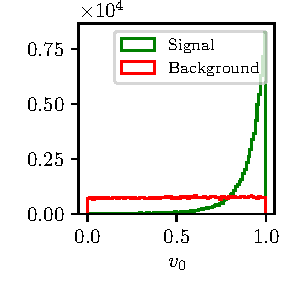
\includegraphics[width=0.241\linewidth]{fig/addendums/QQcC_v0}}
\subfigure{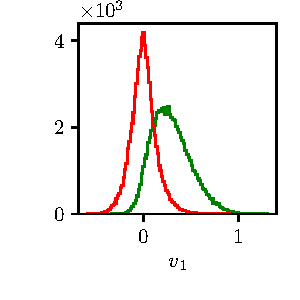
\includegraphics[width=0.241\linewidth]{fig/addendums/QQcC_v1}}
\subfigure{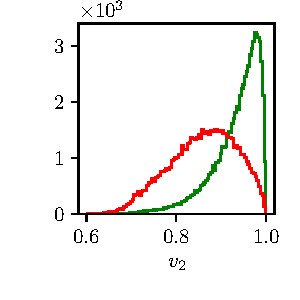
\includegraphics[width=0.241\linewidth]{fig/addendums/QQcC_v2}}
\subfigure{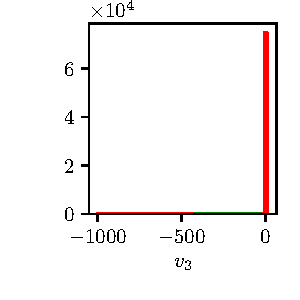
\includegraphics[width=0.241\linewidth]{fig/addendums/QQcC_v3}}\\
\subfigure{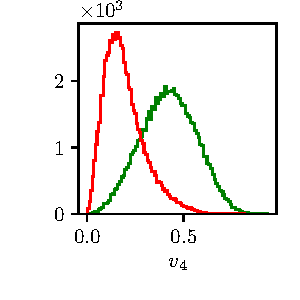
\includegraphics[width=0.241\linewidth]{fig/addendums/QQcC_v4}}
\subfigure{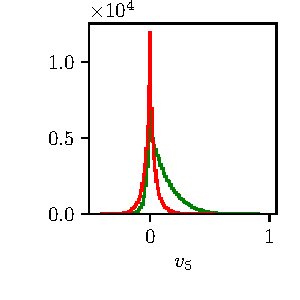
\includegraphics[width=0.241\linewidth]{fig/addendums/QQcC_v5}}
\subfigure{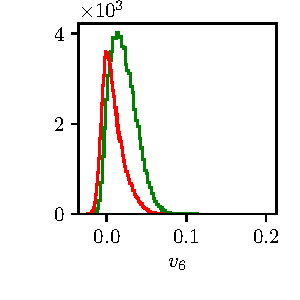
\includegraphics[width=0.241\linewidth]{fig/addendums/QQcC_v6}}
\subfigure{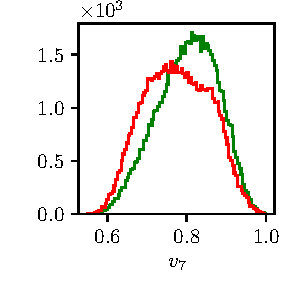
\includegraphics[width=0.241\linewidth]{fig/addendums/QQcC_v7}}\\
\subfigure{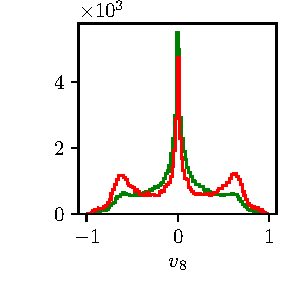
\includegraphics[width=0.241\linewidth]{fig/addendums/QQcC_v8}}
\subfigure{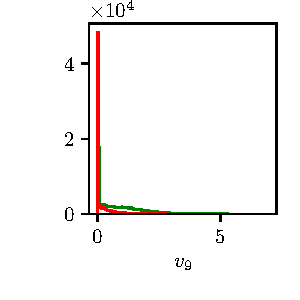
\includegraphics[width=0.241\linewidth]{fig/addendums/QQcC_v9}}
\subfigure{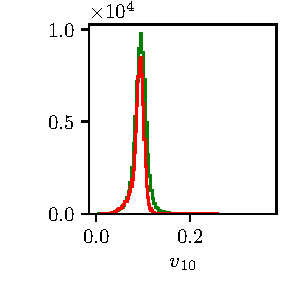
\includegraphics[width=0.241\linewidth]{fig/addendums/QQcC_v10}}
\subfigure{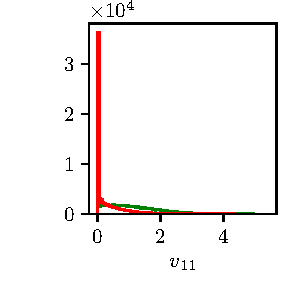
\includegraphics[width=0.241\linewidth]{fig/addendums/QQcC_v11}}\\
\subfigure{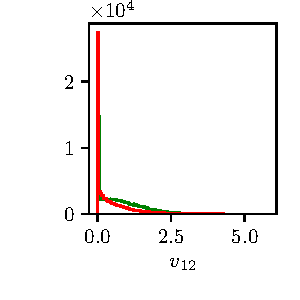
\includegraphics[width=0.241\linewidth]{fig/addendums/QQcC_v12}}
\subfigure{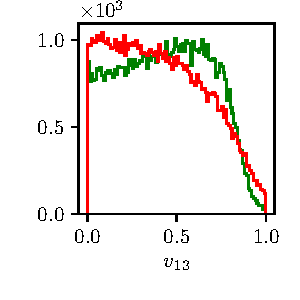
\includegraphics[width=0.241\linewidth]{fig/addendums/QQcC_v13}}
\subfigure{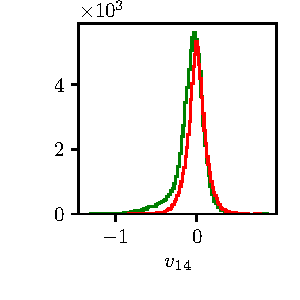
\includegraphics[width=0.241\linewidth]{fig/addendums/QQcC_v14}}
\subfigure{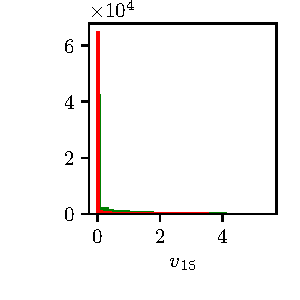
\includegraphics[width=0.241\linewidth]{fig/addendums/QQcC_v15}}\\
\subfigure{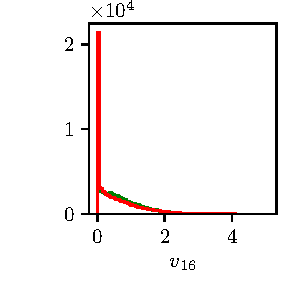
\includegraphics[width=0.241\linewidth]{fig/addendums/QQcC_v16}}
\subfigure{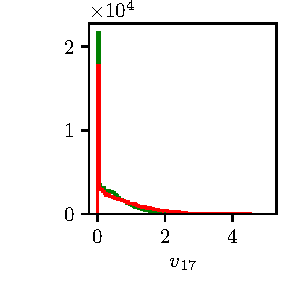
\includegraphics[width=0.241\linewidth]{fig/addendums/QQcC_v17}}
\subfigure{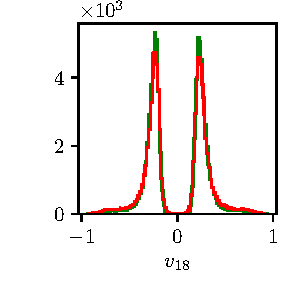
\includegraphics[width=0.241\linewidth]{fig/addendums/QQcC_v18}}
\subfigure{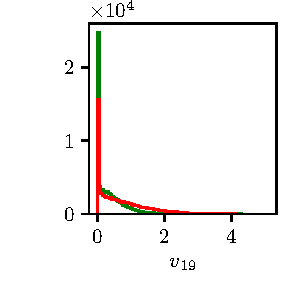
\includegraphics[width=0.241\linewidth]{fig/addendums/QQcC_v19}}
\caption{Feature distributions for MVA training of $q\bar q$ background suppression.}
\end{figure}

\begin{figure}[H]\ContinuedFloat
\captionsetup{width=0.8\linewidth}
\subfigure{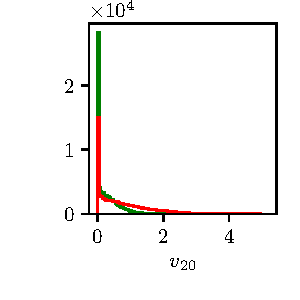
\includegraphics[width=0.241\linewidth]{fig/addendums/QQcC_v20}}
\subfigure{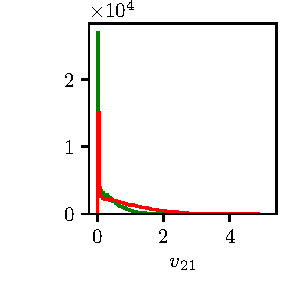
\includegraphics[width=0.241\linewidth]{fig/addendums/QQcC_v21}}
\subfigure{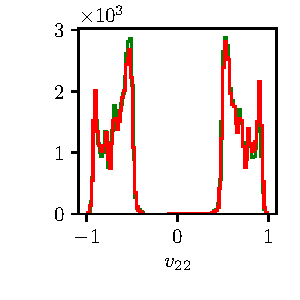
\includegraphics[width=0.241\linewidth]{fig/addendums/QQcC_v22}}
\subfigure{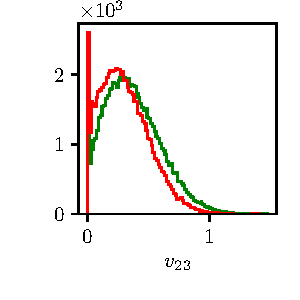
\includegraphics[width=0.241\linewidth]{fig/addendums/QQcC_v23}}\\
\subfigure{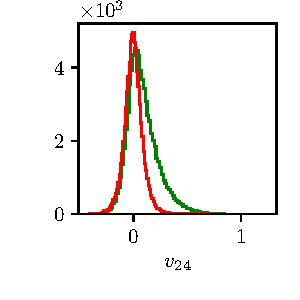
\includegraphics[width=0.241\linewidth]{fig/addendums/QQcC_v24}}
\subfigure{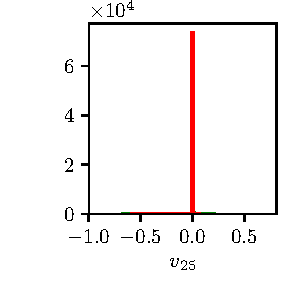
\includegraphics[width=0.241\linewidth]{fig/addendums/QQcC_v25}}
\subfigure{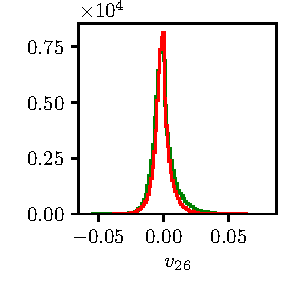
\includegraphics[width=0.241\linewidth]{fig/addendums/QQcC_v26}}
\subfigure{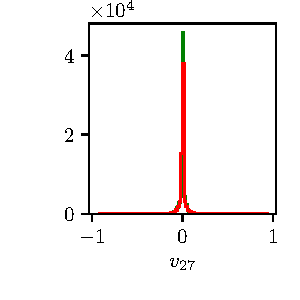
\includegraphics[width=0.241\linewidth]{fig/addendums/QQcC_v27}}\\
\subfigure{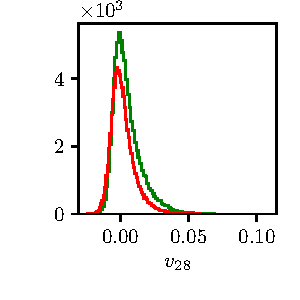
\includegraphics[width=0.241\linewidth]{fig/addendums/QQcC_v28}}
\subfigure{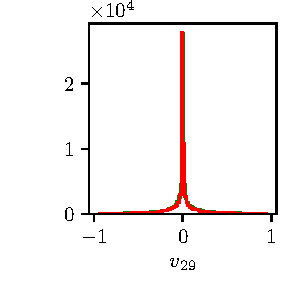
\includegraphics[width=0.241\linewidth]{fig/addendums/QQcC_v29}}
\subfigure{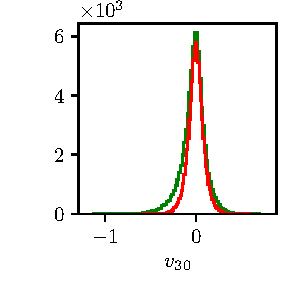
\includegraphics[width=0.241\linewidth]{fig/addendums/QQcC_v30}}
\subfigure{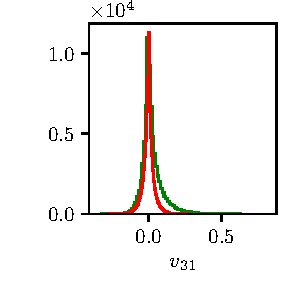
\includegraphics[width=0.241\linewidth]{fig/addendums/QQcC_v31}}\\
\subfigure{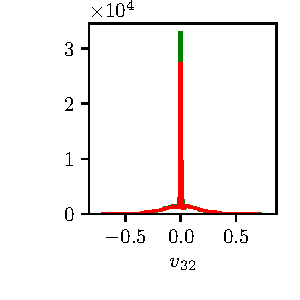
\includegraphics[width=0.241\linewidth]{fig/addendums/QQcC_v32}}
\subfigure{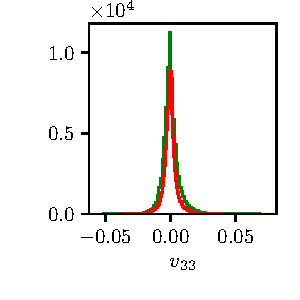
\includegraphics[width=0.241\linewidth]{fig/addendums/QQcC_v33}}
\caption{Feature distributions for MVA training of $q\bar q$ background suppression.}
\end{figure}

\subsection{Hyper-parameter Optimization}

\begin{figure}[H]
\centering
\captionsetup{width=0.8\linewidth}
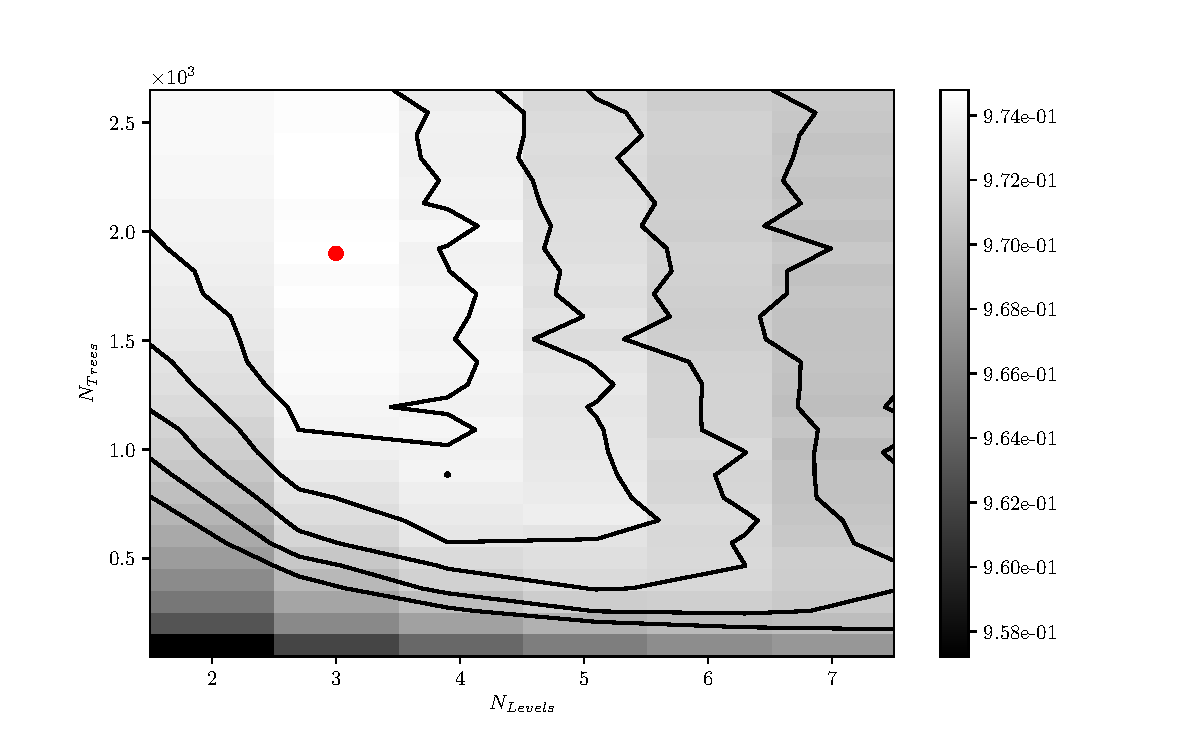
\includegraphics[width=\linewidth]{fig/addendums/QQcC_hpo}
\caption{Hyper-parameter optimization of \texttt{\footnotesize nTrees} and \texttt{\footnotesize nLevels} in the BDT forest training of $q\bar q$ background suppression.}
\end{figure}

\subsection{Results}

\begin{figure}[H]
\centering
\captionsetup{width=0.8\linewidth}
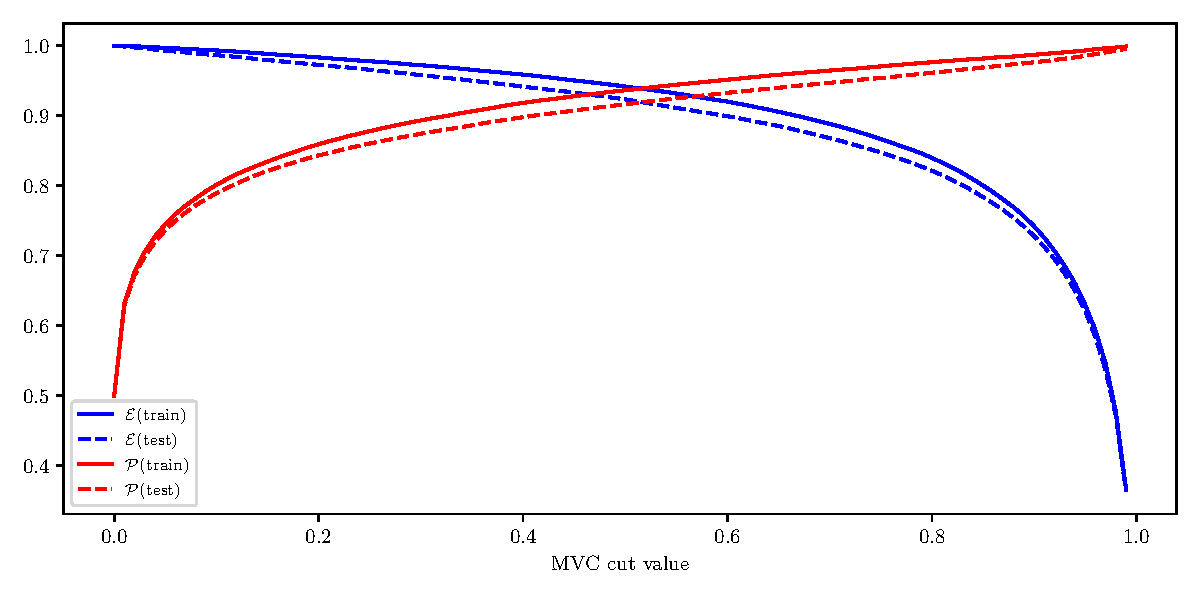
\includegraphics[width=\linewidth]{fig/addendums/QQcC_effpur}
\caption{Efficiency ($\mathcal{E}$) and purity ($\mathcal{P}$) of the MVA classifier output for $q\bar q$ background suppression training on the train (solid) and test (dashed) samples.}
\end{figure}

\begin{figure}[H]
\centering
\captionsetup{width=0.8\linewidth}
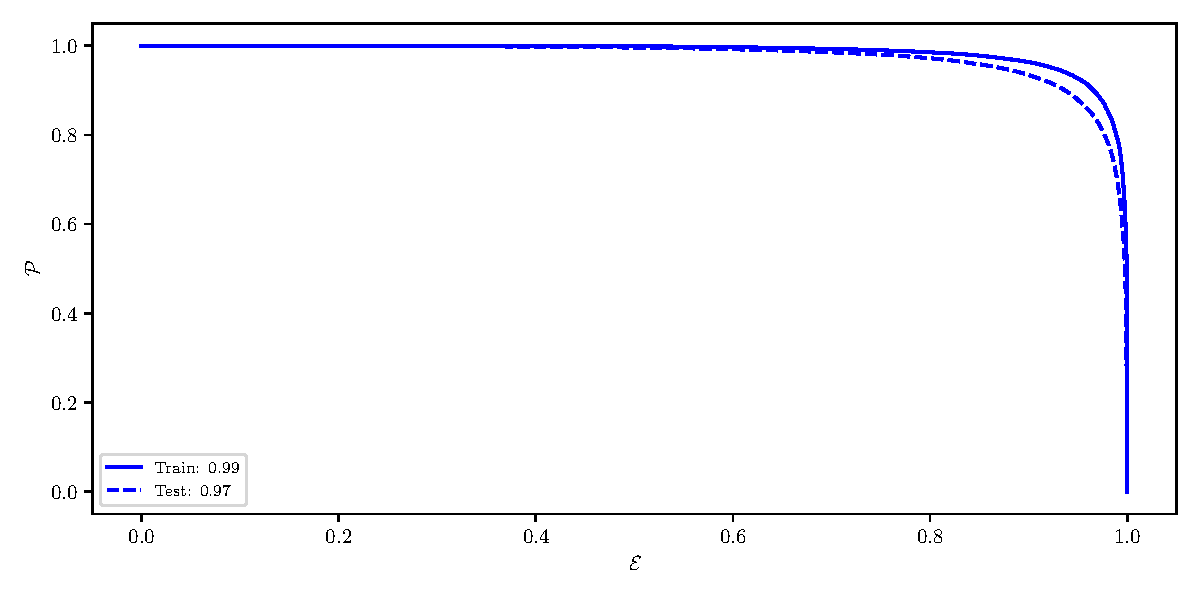
\includegraphics[width=\linewidth]{fig/addendums/QQcC_roc}
\caption{ROC curves of the MVA classifier output for $q\bar q$ background suppression training on the train (solid) and test (dashed) samples.}
\end{figure}

\section{Standard \texorpdfstring{$B \bar B$}{BB-bar} Suppression Training}

\subsection{Variable Importance}

\begin{longtable}{c|l|c|l}
& Name & Alias & Importance \\
\toprule 
0 &\texttt{\footnotesize B\_cosMomVtxKKlnu} & $v_{0}$ & $0.372$ \\ 
1 &\texttt{\footnotesize B\_ROE\_PThetacms0} & $v_{1}$ & $0.096$ \\ 
2 &\texttt{\footnotesize B\_nROETrk0} & $v_{2}$ & $0.079$ \\ 
3 &\texttt{\footnotesize B\_K1FT} & $v_{3}$ & $0.063$ \\ 
4 &\texttt{\footnotesize B\_cosBY} & $v_{4}$ & $0.051$ \\ 
5 &\texttt{\footnotesize B\_roeFit\_dz} & $v_{5}$ & $0.047$ \\ 
6 &\texttt{\footnotesize B\_xiZ0} & $v_{6}$ & $0.043$ \\ 
7 &\texttt{\footnotesize B\_cosMomVtx} & $v_{7}$ & $0.038$ \\ 
8 &\texttt{\footnotesize B\_chiProb} & $v_{8}$ & $0.031$ \\ 
9 &\texttt{\footnotesize B\_nKaonInROE} & $v_{9}$ & $0.028$ \\ 
10 &\texttt{\footnotesize B\_missM2Veto1} & $v_{10}$ & $0.026$ \\ 
11 &\texttt{\footnotesize B\_missM2Veto2} & $v_{11}$ & $0.021$ \\ 
12 &\texttt{\footnotesize B\_nROEDistTrk} & $v_{12}$ & $0.018$ \\ 
13 &\texttt{\footnotesize B\_cosMomVtxKK} & $v_{13}$ & $0.018$ \\ 
14 &\texttt{\footnotesize B\_K0FT} & $v_{14}$ & $0.017$ \\ 
15 &\texttt{\footnotesize B\_QVeto1} & $v_{15}$ & $0.016$ \\ 
16 &\texttt{\footnotesize B\_missM20} & $v_{16}$ & $0.015$ \\ 
17 &\texttt{\footnotesize B\_TagVPvalue} & $v_{17}$ & $0.012$ \\ 
18 &\texttt{\footnotesize B\_QVeto2} & $v_{18}$ & $0.010$ \\ 
\bottomrule
\captionsetup{width=0.8\linewidth}
\caption{Variable names, aliases and importance in the scope of $B\bar B$ background suppression.}
\end{longtable}

\subsection{Variable Distributions}

\begin{figure}[H]
\centering
\captionsetup{width=0.8\linewidth}
\subfigure{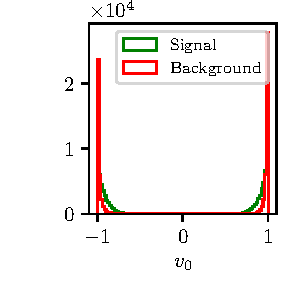
\includegraphics[width=0.241\linewidth]{fig/addendums/BBcC_v0}}
\subfigure{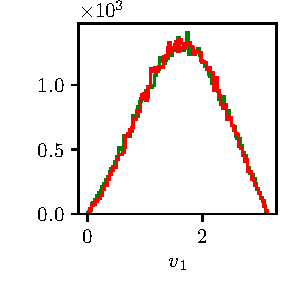
\includegraphics[width=0.241\linewidth]{fig/addendums/BBcC_v1}}
\subfigure{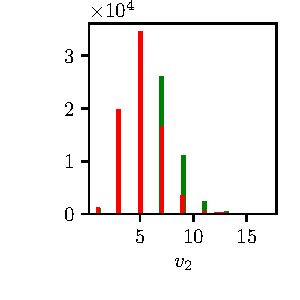
\includegraphics[width=0.241\linewidth]{fig/addendums/BBcC_v2}}
\subfigure{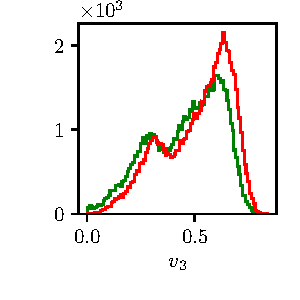
\includegraphics[width=0.241\linewidth]{fig/addendums/BBcC_v3}}\\
\subfigure{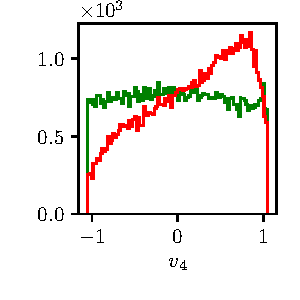
\includegraphics[width=0.241\linewidth]{fig/addendums/BBcC_v4}}
\subfigure{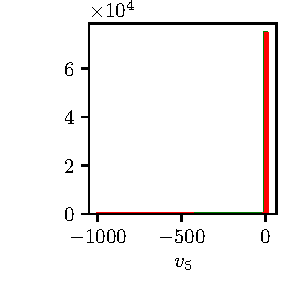
\includegraphics[width=0.241\linewidth]{fig/addendums/BBcC_v5}}
\subfigure{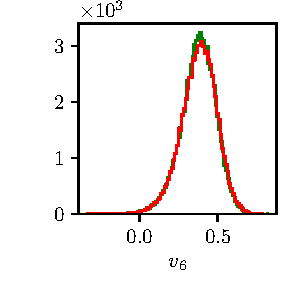
\includegraphics[width=0.241\linewidth]{fig/addendums/BBcC_v6}}
\subfigure{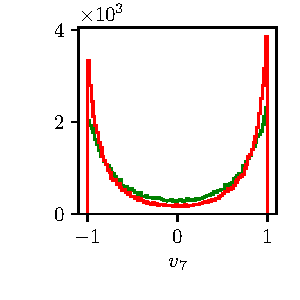
\includegraphics[width=0.241\linewidth]{fig/addendums/BBcC_v7}}\\
\subfigure{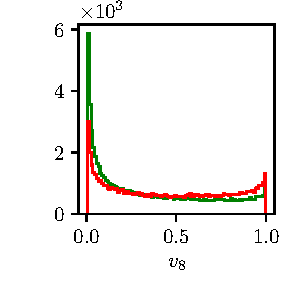
\includegraphics[width=0.241\linewidth]{fig/addendums/BBcC_v8}}
\subfigure{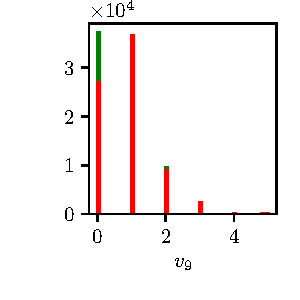
\includegraphics[width=0.241\linewidth]{fig/addendums/BBcC_v9}}
\subfigure{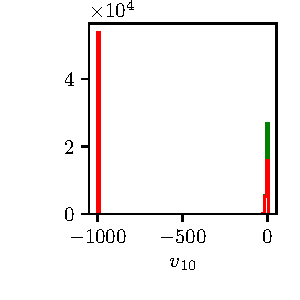
\includegraphics[width=0.241\linewidth]{fig/addendums/BBcC_v10}}
\subfigure{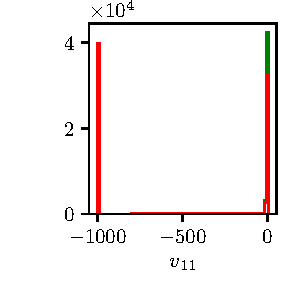
\includegraphics[width=0.241\linewidth]{fig/addendums/BBcC_v11}}\\
\subfigure{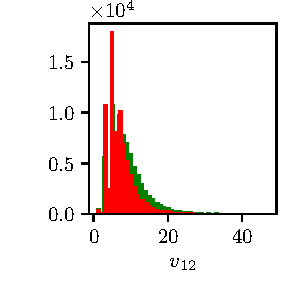
\includegraphics[width=0.241\linewidth]{fig/addendums/BBcC_v12}}
\subfigure{\includegraphics[width=0.241\linewidth]{fig/addendums/BBcC_v13}}
\subfigure{\includegraphics[width=0.241\linewidth]{fig/addendums/BBcC_v14}}
\subfigure{\includegraphics[width=0.241\linewidth]{fig/addendums/BBcC_v15}}\\
\subfigure{\includegraphics[width=0.241\linewidth]{fig/addendums/BBcC_v16}}
\subfigure{\includegraphics[width=0.241\linewidth]{fig/addendums/BBcC_v17}}
\subfigure{\includegraphics[width=0.241\linewidth]{fig/addendums/BBcC_v18}}
\caption{Feature distributions for MVA training of $B\bar B$ background suppression.}
\end{figure}

\subsection{Hyper-parameter Optimization}

\begin{figure}[H]
\centering
\captionsetup{width=0.8\linewidth}
\includegraphics[width=\linewidth]{fig/addendums/BBcC_hpo}
\caption{Hyper-parameter optimization of \texttt{\footnotesize nTrees} and \texttt{\footnotesize nLevels} in the BDT forest training of $B\bar B$ background suppression.}
\end{figure}

\subsection{Results}

\begin{figure}[H]
\centering
\captionsetup{width=0.8\linewidth}
\includegraphics[width=\linewidth]{fig/addendums/BBcC_effpur}
\caption{Efficiency ($\mathcal{E}$) and purity ($\mathcal{P}$) of the MVA classifier output for $B\bar B$ background suppression training on the train (solid) and test (dashed) samples.}
\end{figure}

\begin{figure}[H]
\centering
\captionsetup{width=0.8\linewidth}
\includegraphics[width=\linewidth]{fig/addendums/BBcC_roc}
\caption{ROC curves of the MVA classifier output for $B\bar B$ background suppression training on the train (solid) and test (dashed) samples.}
\end{figure}

\section{Uniformity Boosted \texorpdfstring{$B \bar B$}{BB-bar} Suppression Training}

\subsection{Hyper-parameter Optimization}

Hyper-parameters were not optimized due to the large CPU time consumption of the algorithm. The following set up of the hyper-parameters was chosen
\begin{itemize}
\item \texttt{\footnotesize nTrees}: 300
\item \texttt{\footnotesize nLevels}: 4
\end{itemize}

\subsection{Results}

\begin{figure}[H]
\centering
\captionsetup{width=0.8\linewidth}
\includegraphics[width=\linewidth]{fig/addendums/uBBcC_effpur}
\caption{Efficiency ($\mathcal{E}$) and purity ($\mathcal{P}$) of the uniformity boosted MVA classifier output for $B\bar B$ background suppression training on the train (solid) and test (dashed) samples.}
\end{figure}

\begin{figure}[H]
\centering
\captionsetup{width=0.8\linewidth}
\includegraphics[width=\linewidth]{fig/addendums/uBBcC_roc}
\caption{ROC curves of the uniformity boosted MVA classifier output for $B\bar B$ background suppression training on the train (solid) and test (dashed) samples.}
\end{figure}